% =====================================================================
%  Presentazione finale - Analisi di Social Network e Media
%  CdLM in Ingegneria Informatica - DIMES, Universita' della Calabria
%
%  Compilazione:  pdflatex presentazione.tex   (due volte, per i numeri di pagina)
%  Le figure stanno in figure/ (le stesse della relazione, in PDF).
%  Stesso tema della proposta, cosi' il deck si legge come continuazione.
% =====================================================================
\documentclass[aspectratio=169,10pt]{beamer}

\usepackage[utf8]{inputenc}
\usepackage[T1]{fontenc}
\usepackage{lmodern}
\usepackage[italian]{babel}
\usepackage{amsmath,amssymb}
\usepackage{booktabs}
\usepackage{array,colortbl}
\usepackage{graphicx}
\usepackage{tikz}
\usetikzlibrary{arrows.meta,positioning,calc}

\graphicspath{{figure/}}

% ------------------------------------------------- aspetto
\usetheme{default}
\setbeamertemplate{navigation symbols}{}
\setbeamertemplate{itemize items}[circle]
\setbeamertemplate{caption}{\insertcaption}

\definecolor{petrolio}{RGB}{15,107,99}
\definecolor{petrolioscuro}{RGB}{11,83,77}
\definecolor{bordeaux}{RGB}{138,31,61}
\definecolor{ambra}{RGB}{138,90,18}
\definecolor{inchiostro}{RGB}{20,24,26}
\definecolor{grigio}{RGB}{110,118,121}
\definecolor{grigiochiaro}{RGB}{236,239,238}
\definecolor{tenue}{RGB}{220,235,233}
\definecolor{tenuebord}{RGB}{246,226,232}

\setbeamercolor{structure}{fg=petrolio}
\setbeamercolor{normal text}{fg=inchiostro}
\setbeamercolor{frametitle}{fg=petrolioscuro}
\setbeamercolor{title}{fg=petrolioscuro}
\setbeamercolor{block title}{bg=tenue,fg=petrolioscuro}
\setbeamercolor{block body}{bg=grigiochiaro,fg=inchiostro}
\setbeamercolor{alerted text}{fg=bordeaux}
\setbeamerfont{frametitle}{size=\large,series=\bfseries}
\setbeamerfont{title}{size=\LARGE,series=\bfseries}

\setbeamertemplate{frametitle}{%
  \vspace*{0.6em}\hspace*{0.9em}%
  \begin{minipage}{0.92\textwidth}
    \usebeamerfont{frametitle}\usebeamercolor[fg]{frametitle}\insertframetitle%
    \ifx\insertframesubtitle\@empty\else
      \\[0.15em]{\usebeamerfont{framesubtitle}\color{grigio}\small\insertframesubtitle}%
    \fi
  \end{minipage}%
  \vspace*{0.3em}%
  \hrule height 0.6pt width \paperwidth
}
\setbeamertemplate{footline}{%
  \hbox{\begin{beamercolorbox}[wd=\paperwidth,ht=2.4ex,dp=1.2ex,leftskip=1em,rightskip=1em]{}%
    {\color{grigio}\scriptsize Relazione finale \textperiodcentered{} ASNM
     \hfill \insertframenumber/\inserttotalframenumber}%
  \end{beamercolorbox}}%
}

% scorciatoie
\newcommand{\slabel}[1]{{\color{grigio}\scriptsize\textsc{#1}}}
\newcommand{\grande}[1]{{\fontsize{26}{30}\selectfont\bfseries\color{petrolioscuro}#1}}
\newcommand{\grandeb}[1]{{\fontsize{20}{24}\selectfont\bfseries\color{bordeaux}#1}}
\newcommand{\male}[1]{{\color{bordeaux}#1}}
\newcommand{\pos}[1]{{\color{petrolioscuro}#1}}
\newcommand{\Qtras}{Q_{\mathrm{tras}}}
\newcommand{\phat}{\hat{p}}

\title{Massimizzazione dell'influenza con vincolo di diversit\`a\\
       su rete multistrato}
\subtitle{Dal cancello sul substrato alla previsione di chi adotter\`a}
\author{Davide Cinelli \and Giuseppe Cuiuri}
\institute{Analisi di Social Network e Media\\
           CdLM in Ingegneria Informatica \textperiodcentered{} DIMES,
           Universit\`a della Calabria\\[0.4em]
           \small Docente: prof.\ Andrea Tagarelli}
\date{Settembre 2026}

\begin{document}

% =====================================================================
\begin{frame}[plain]
  \titlepage
\end{frame}

% =====================================================================
\begin{frame}{Due domande}
  \begin{columns}[T]
    \begin{column}{0.48\textwidth}
      \slabel{la domanda di previsione}\\[0.3em]
      {\large\bfseries Chi adotter\`a?}\\[1.2em]
      \slabel{la domanda di ottimizzazione}\\[0.3em]
      {\large\bfseries Da chi conviene partire?}\\[1.2em]
      \small Il progetto \`e nato dalla seconda.\\
      Misurando, la domanda centrale \`e diventata la prima.
    \end{column}
    \begin{column}{0.48\textwidth}
      \begin{alertblock}{La difficolt\`a non sono gli algoritmi}
        \small Nella quasi totalit\`a dei lavori di IM le probabilit\`a sono assegnate e i seed valutati sotto lo stesso modello che li ha scelti. Il ciclo si autoconferma.
      \end{alertblock}
    \end{column}
  \end{columns}
\end{frame}

% =====================================================================
\begin{frame}{Due dataset, due situazioni opposte}
  \begin{columns}[T]
    \begin{column}{0.52\textwidth}
      \scriptsize
      \begin{tabular}{@{}lll@{}}
        \toprule
         & \textbf{StackExchange} & \textbf{Higgs Twitter} \\
        \midrule
        canale & risposte, commenti & grafo dei follower \\
        nodi & 46.312 & 456.627 \\
        archi & 230.641 & 14.855.842 \\
        livelli & 2 & 4 \\
        oggetto & 105 tag, 12 anni & un evento, 7 giorni \\
        confine & gennaio 2020 & ora 72 \\
        da prevedere & 64.711 esposizioni & 269.081 adottanti \\
        \midrule
        \textbf{eccesso strutturale} & \male{$\mathbf{-0\%}$} & \pos{$\mathbf{+73\%}$} \\
        \bottomrule
      \end{tabular}
    \end{column}
    \begin{column}{0.46\textwidth}
      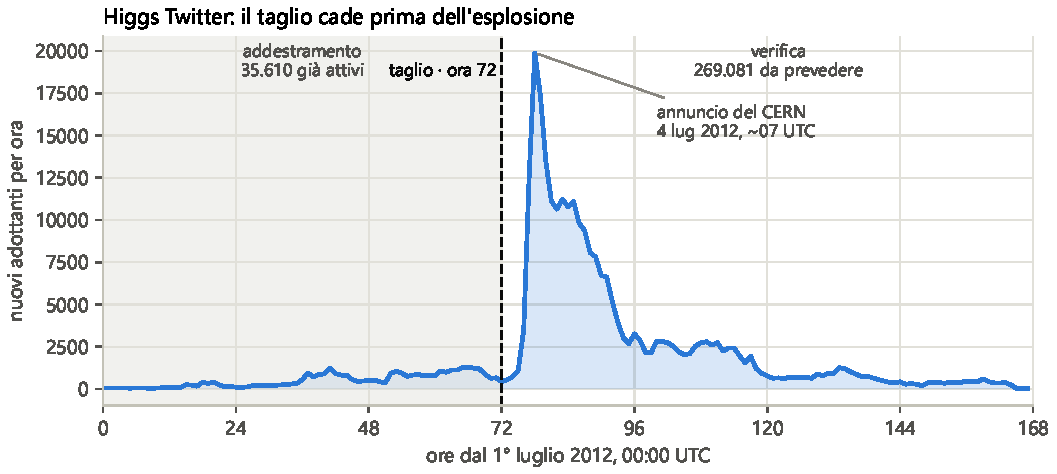
\includegraphics[width=\textwidth]{fig_adozioni_ora}
      \vspace{0.3em}
      \small Il taglio cade \emph{poche ore prima} dell'annuncio del CERN: i seed si scelgono quando l'evento non \`e ancora esploso.
    \end{column}
  \end{columns}
\end{frame}

% =====================================================================
\begin{frame}{Il cancello: la rete conta, qui?}{Una misura decisa prima di costruire qualunque cosa}
  \begin{columns}[T]
    \begin{column}{0.55\textwidth}
      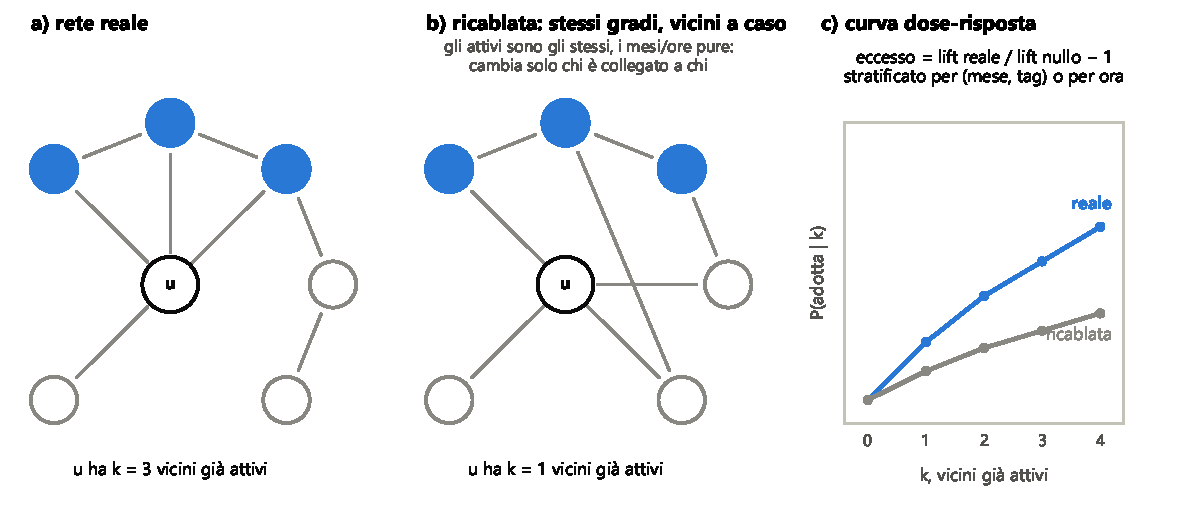
\includegraphics[width=\textwidth]{schema_dose}
    \end{column}
    \begin{column}{0.43\textwidth}
      \small
      Se i tuoi vicini hanno adottato, tu adotti di pi\`u. Ma chi ha molti vicini \`e pi\`u attivo.\\[0.6em]
      Si confronta la rete reale con reti \textbf{ricablate a gradi preservati}: stessi nodi, stesso numero di vicini, vicini diversi.
      \[
        \text{eccesso} = \frac{\text{lift reale}}{\text{lift nullo}} - 1
      \]
      \textbf{Stratificato} per (mese, tag) o per ora: nei momenti di picco tutti sono esposti e tutti adottano, e il rapporto aggregato lo scambia per rete.\\[0.6em]
      \alert{Soglia $+40\%$, fissata prima di misurare.}
    \end{column}
  \end{columns}
\end{frame}

% =====================================================================
\begin{frame}{Il cancello: il verdetto in entrambe le direzioni}
  \begin{columns}[T]
    \begin{column}{0.55\textwidth}
      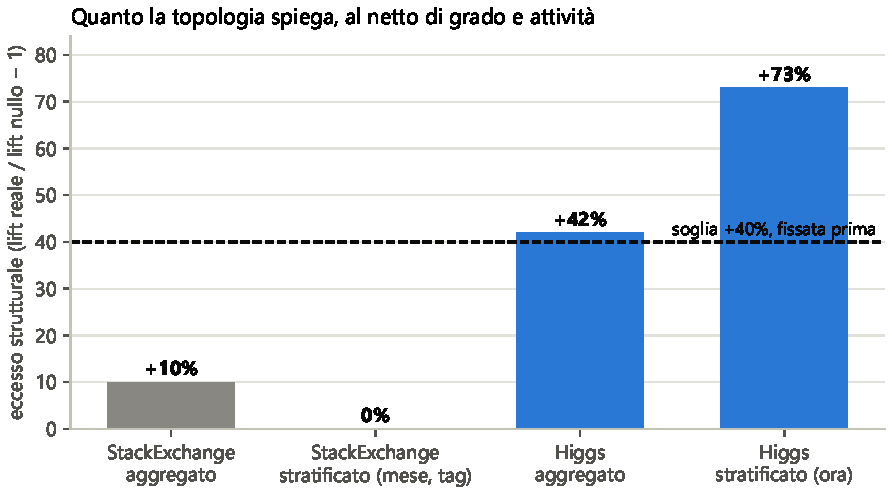
\includegraphics[width=\textwidth]{fig_eccesso}
    \end{column}
    \begin{column}{0.43\textwidth}
      \small
      \textbf{StackExchange}: il $+10\%$ aggregato \male{sparisce} stratificando --- 1,54$\times$ reale contro 1,54$\times$ nullo. Era composizione del campione.\\[0.5em]
      \textbf{Higgs}: $+42\%$ aggregato, \pos{$+73\%$} stratificato.\\[0.8em]
      \begin{block}{Che cosa spiega}
        Ogni risultato nullo della prima versione --- GNN, diversit\`a, competitivo --- non era un difetto di implementazione: non c'era struttura da trovare.
      \end{block}
      StackExchange resta come \textbf{controllo negativo}.
    \end{column}
  \end{columns}
\end{frame}

% =====================================================================
\begin{frame}{L'architettura}
  \centering
  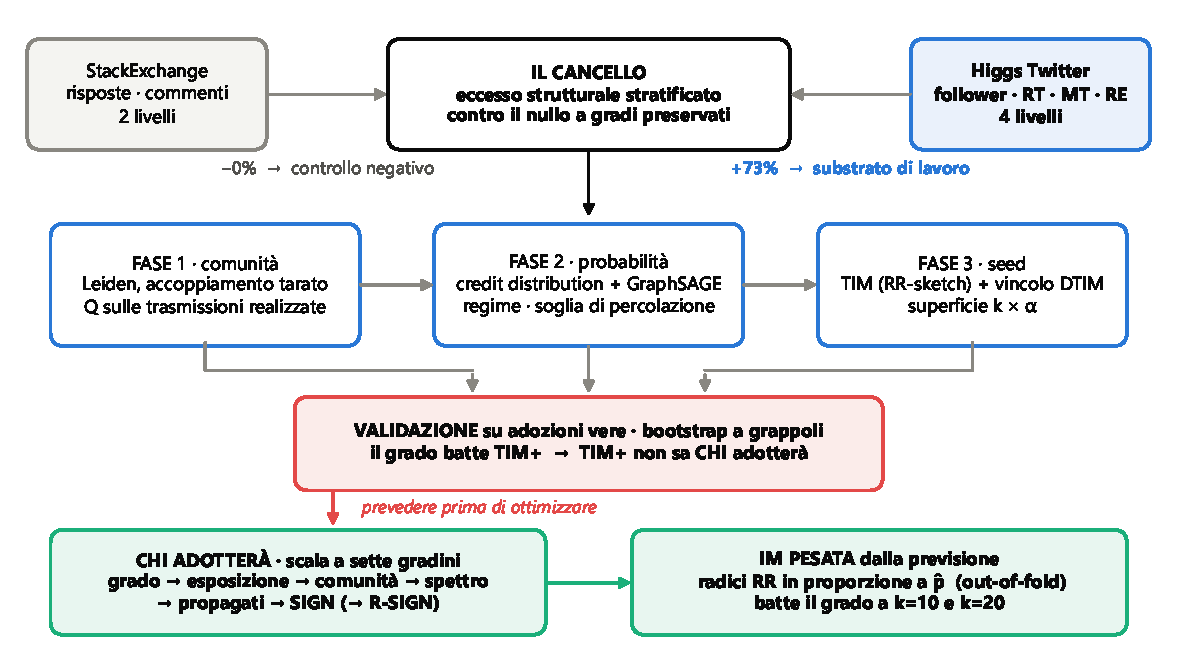
\includegraphics[width=0.92\textwidth]{fig_architettura}
\end{frame}

% =====================================================================
\begin{frame}{Fase 1 --- le comunit\`a predicono dove passa la diffusione}{Criterio fuori campione: modularit\`a sulle trasmissioni realizzate \emph{dopo} il taglio}
  \begin{columns}[T]
    \begin{column}{0.55\textwidth}
      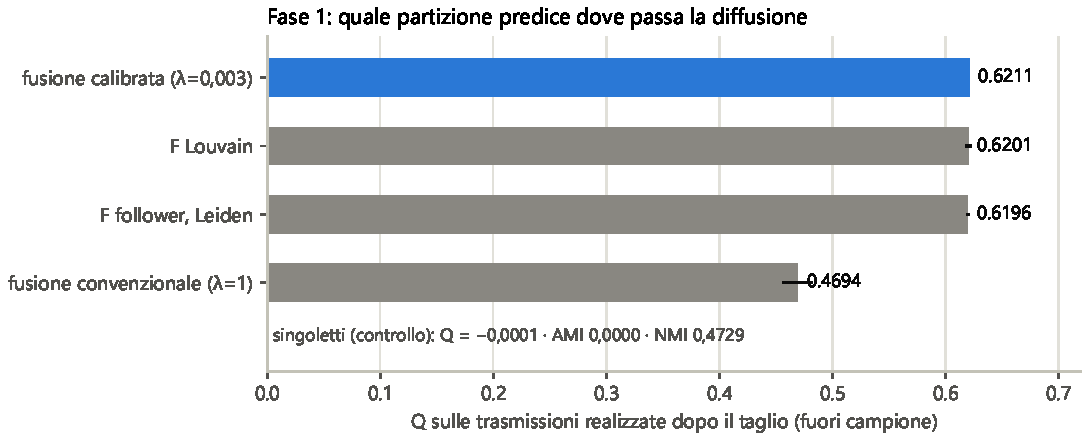
\includegraphics[width=\textwidth]{fig_fase1_q}
    \end{column}
    \begin{column}{0.43\textwidth}
      \small
      \grande{$\Qtras = 0{,}62$}\\
      contro 0,13 su StackExchange; il 74\% delle 5,6 M trasmissioni resta dentro la comunit\`a, 7$\times$ il caso.\\[0.8em]
      \textbf{Leiden $\equiv$ Louvain} ($p = 0{,}19$).\\[0.4em]
      \textbf{Il multistrato paga solo tarato}: con la normalizzazione convenzionale la fusione crolla a 0,47; con il peso degli strati scelto in campione ($\lambda = 0{,}003$) vince, $p < 0{,}001$.\\[0.4em]
      Il verdetto sul multistrato dipende da una scelta che di solito non viene dichiarata.
    \end{column}
  \end{columns}
\end{frame}

% =====================================================================
\begin{frame}{Fase 1 --- la trappola della metrica}
  \begin{columns}[T]
    \begin{column}{0.45\textwidth}
      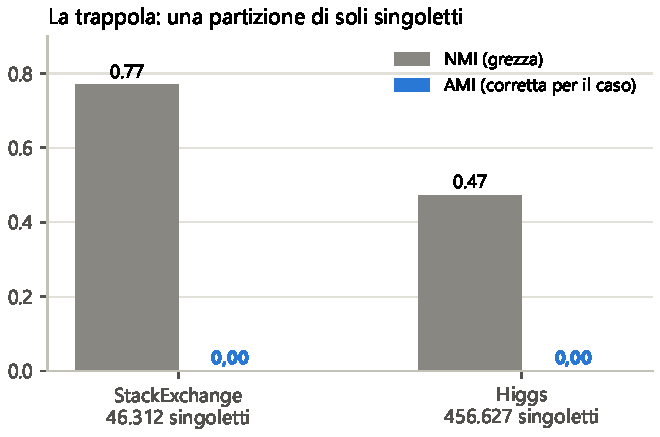
\includegraphics[width=\textwidth]{fig_nmi_ami}
    \end{column}
    \begin{column}{0.52\textwidth}
      \small
      Una partizione di \textbf{soli singoletti} --- ogni nodo da solo, nessuna struttura ---\\[0.5em]
      \begin{tabular}{@{}lrr@{}}
        \toprule
         & StackExchange & Higgs \\
        \midrule
        NMI (grezza) & \male{0,77} & \male{0,47} \\
        AMI (corretta per il caso) & \pos{0,00} & \pos{0,00} \\
        $Q$ (nullo dentro) & $-0{,}004$ & $-0{,}0001$ \\
        \bottomrule
      \end{tabular}\\[0.8em]
      L'NMI non sottrae l'accordo casuale e premia la granularit\`a come se fosse accuratezza. Riprodotto su due substrati.\\[0.5em]
      \alert{Ogni metrica del lavoro ha il modello nullo dentro.}
    \end{column}
  \end{columns}
\end{frame}

% =====================================================================
\begin{frame}{Fase 2 --- probabilit\`a stimate, non assegnate}
  \begin{columns}[T]
    \begin{column}{0.5\textwidth}
      \small
      \textbf{Credit distribution}, orientata, sui retweet \emph{osservati}:
      \[
        p(u \to v) = \frac{\text{trasmissioni}(u \to v)}{\text{attivit\`a}(u) + s}
      \]
      28.498 archi con dati su 14,8 M --- lo 0,19\%.\\[0.6em]
      \textbf{GraphSAGE} estende la stima agli altri:\\[0.3em]
      \begin{tabular}{@{}lrr@{}}
        \toprule
        modello di $p$ & MSE & vs costante \\
        \midrule
        loss uniforme & 0,000222 & \pos{$-86\%$} \\
        loss pesata sugli hub & 0,000261 & \male{$-2{,}1\%$ sugli hub} \\
        costante & 0,001588 & --- \\
        \bottomrule
      \end{tabular}\\[0.5em]
      La loss pesata \`e respinta \textbf{su entrambi i substrati} ($-2{,}1\%$ e $-2{,}0\%$): una replica, non un secondo tentativo.
    \end{column}
    \begin{column}{0.48\textwidth}
      \begin{block}{Due scelte}
        \small
        \begin{itemize}
          \item un solo verso per arco: il verso opposto non \`e «influenza zero», \`e assenza di canale
          \item quattro archi \emph{negativi} per ogni ricco, o la rete sovrastima sui poveri
        \end{itemize}
      \end{block}
    \end{column}
  \end{columns}
\end{frame}

% =====================================================================
\begin{frame}{Fase 2 --- la soglia di percolazione, e l'annuncio che la attraversa}
  \begin{columns}[T]
    \begin{column}{0.5\textwidth}
      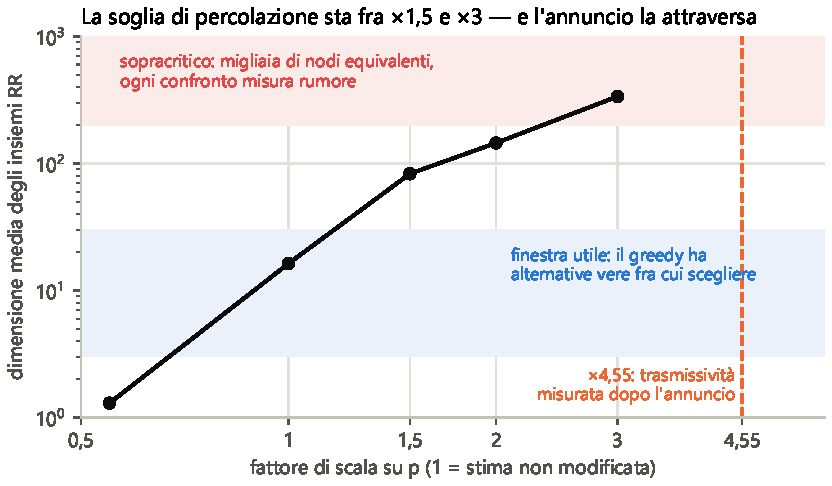
\includegraphics[width=\textwidth]{fig_regime}
    \end{column}
    \begin{column}{0.5\textwidth}
      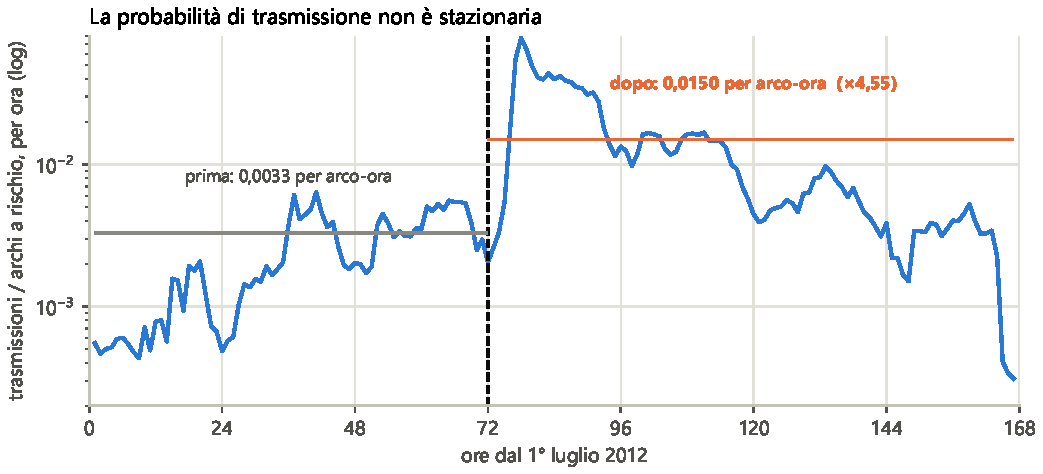
\includegraphics[width=\textwidth]{fig_stazionarieta}
    \end{column}
  \end{columns}
  \vspace{0.4em}
  \small
  Alla scala 1 --- la stima non modificata --- il sistema \`e sottocritico: \textbf{nessuna riscalatura} (su StackExchange serviva 0,25). La soglia sta fra $\times 1{,}5$ e $\times 3$. Dopo l'annuncio la trasmissivit\`a per arco-ora sale di \textbf{4,55$\times$}: \textbf{nel periodo calmo la rete non percola, l'annuncio la spinge sopra soglia.} L'esplosione non \`e arrivata dalla rete; la rete l'ha amplificata.
\end{frame}

% =====================================================================
\begin{frame}{Fase 3 --- quanto costa la diversit\`a}{$s(v) = \alpha \cdot |R_v| / \max_u |R_u| + (1-\alpha)\cdot \mathbf{1}[c(v) \notin C]$}
  \begin{columns}[T]
    \begin{column}{0.58\textwidth}
      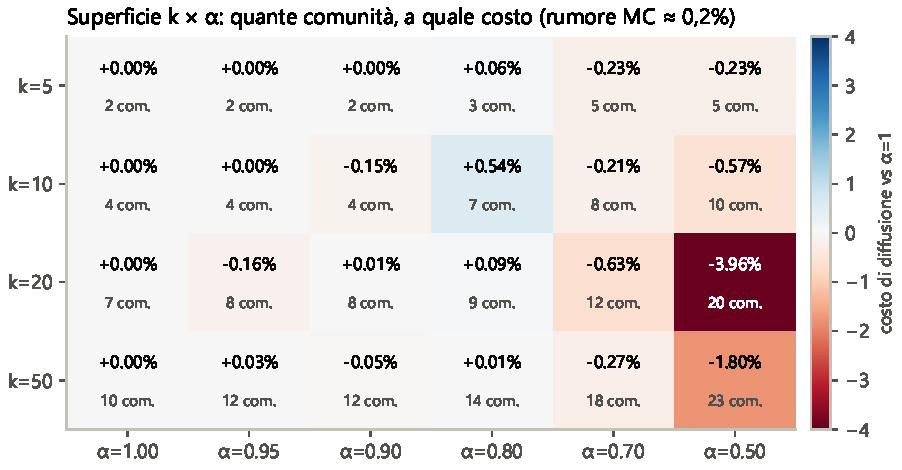
\includegraphics[width=\textwidth]{fig_superficie}
    \end{column}
    \begin{column}{0.4\textwidth}
      \small
      Rumore Monte Carlo sulla differenza fra due celle: $\approx 0{,}2\%$.\\[0.6em]
      A $k = 50$: da 10 a \textbf{14 comunit\`a gratis}, a 18 per lo 0,27\%, tutte e 23 per l'1,8\%.\\[0.4em]
      A $k = 10$: da 4 a 7 comunit\`a \pos{$+0{,}54\%$} --- spargere i seed riduce la sovrapposizione.\\[0.8em]
      Su StackExchange la stessa mossa a $k=5$ costava l'1,35\% e apriva comunit\`a da due nodi. Qui il vincolo ha 23 comunit\`a bilanciate su cui lavorare.
    \end{column}
  \end{columns}
\end{frame}

% =====================================================================
\begin{frame}{La validazione}{Punteggio $= \sum_v \pi(v)$ sui 269.081 veri adottanti; bootstrap a grappoli sull'ora}
  \begin{columns}[T]
    \begin{column}{0.55\textwidth}
      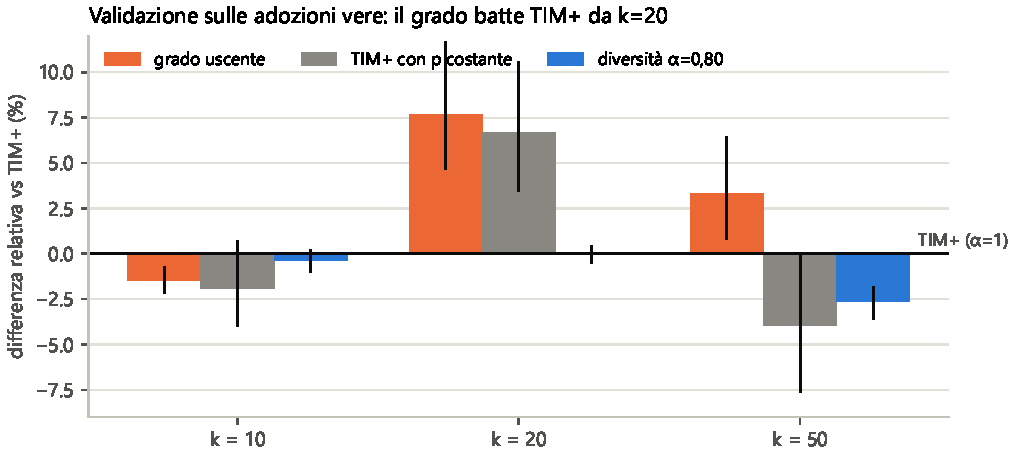
\includegraphics[width=\textwidth]{fig_validazione}
    \end{column}
    \begin{column}{0.43\textwidth}
      \grandeb{Il grado batte TIM+}\\[0.3em]
      \small $+7{,}66\%$ a $k=20$, $+3{,}34\%$ a $k=50$, $p \le 0{,}001$. Regge anche a $\times 4{,}55$.\\[0.6em]
      Credit distribution, GraphSAGE, RR-sketch e greedy con garanzia $1-1/e$ perdono contro «prendi i venti account con pi\`u follower».\\[0.6em]
      Non \`e rumore: il modello batte il caso del 24--98\%. \`E che \textbf{TIM+ massimizza \emph{quanti}, e non sa \emph{quali}}.\\[0.6em]
      \pos{Il vincolo di diversit\`a \`e gratis}: $-0{,}02\%$ a $k=20$, $p = 0{,}93$.
    \end{column}
  \end{columns}
\end{frame}

% =====================================================================
\begin{frame}{Chi adotter\`a --- la scala a pioli}{Sui 421.017 non attivi all'ora 72: chi adotta nelle 96 ore dopo?}
  \begin{columns}[T]
    \begin{column}{0.55\textwidth}
      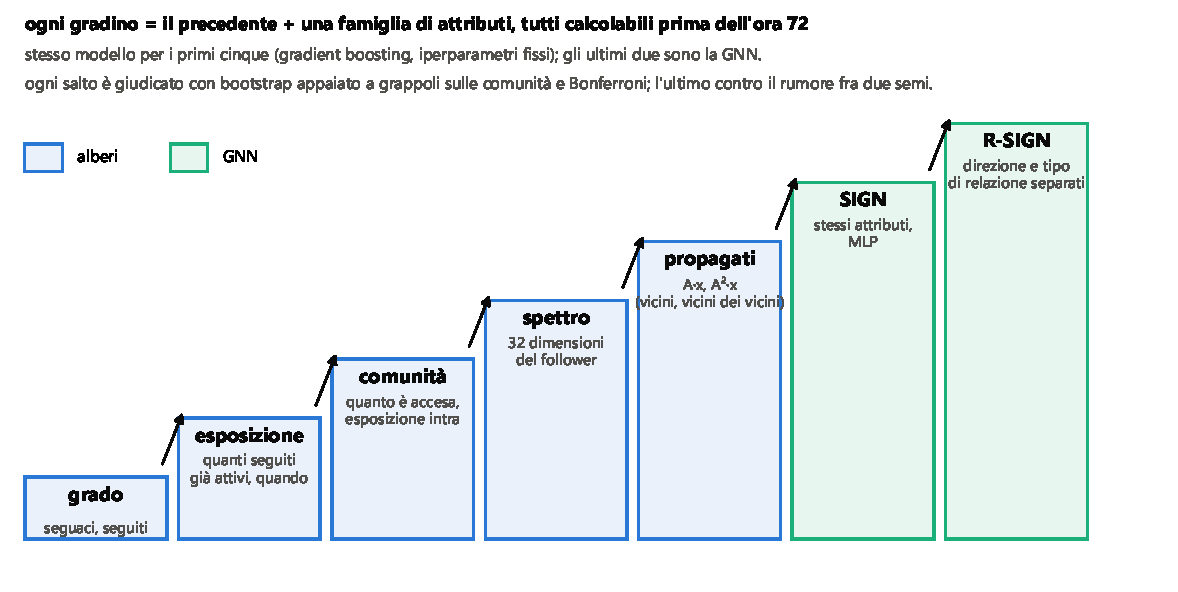
\includegraphics[width=\textwidth]{schema_scala}
    \end{column}
    \begin{column}{0.43\textwidth}
      \small
      Ogni gradino = il precedente + una famiglia di attributi, tutti pre-taglio. Stesso modello per i primi cinque; gli ultimi due sono la GNN.\\[0.6em]
      Le comunit\`a entrano come \textbf{numeri} --- quanto \`e accesa la mia, quanta esposizione viene da dentro --- non come identit\`a.\\[0.6em]
      Ogni salto: bootstrap a grappoli \textbf{sulle comunit\`a}, Bonferroni, e il rumore fra due semi come metro dell'ultimo.
    \end{column}
  \end{columns}
\end{frame}

% =====================================================================
\begin{frame}{Chi adotter\`a --- cinque salti, cinque positivi}
  \begin{columns}[T]
    \begin{column}{0.6\textwidth}
      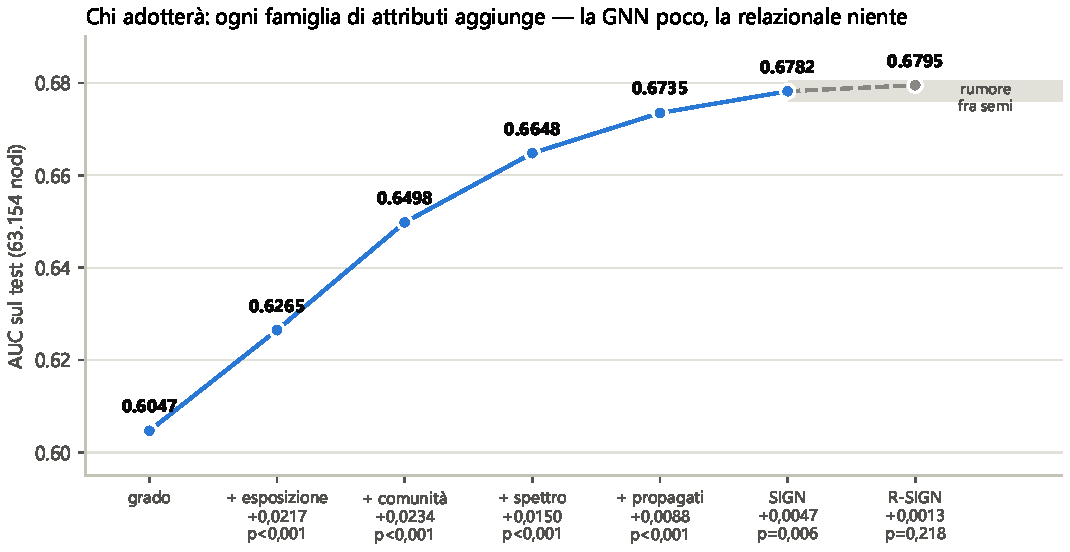
\includegraphics[width=\textwidth]{fig_scala}
    \end{column}
    \begin{column}{0.38\textwidth}
      \small
      \begin{tabular}{@{}lr@{}}
        \toprule
        salto & $\Delta$AUC \\
        \midrule
        grado $\to$ esposizione & $+0{,}022$ \\
        $\to$ \textbf{comunit\`a} & \pos{$\mathbf{+0{,}023}$} \\
        $\to$ spettro & $+0{,}015$ \\
        $\to$ propagati & $+0{,}009$ \\
        $\to$ SIGN & $+0{,}005$ \\
        $\to$ R-SIGN & \male{$+0{,}001$, n.s.} \\
        \bottomrule
      \end{tabular}\\[0.6em]
      Tutti i primi cinque sotto Bonferroni. \textbf{Le comunit\`a sono il gradino pi\`u grande.} La GNN aggiunge poco ma davvero; la struttura relazionale informa gli alberi, non la GNN.\\[0.4em]
      AUC finale 0,68: modesta, e va detto.
    \end{column}
  \end{columns}
\end{frame}

% =====================================================================
\begin{frame}{IM pesata dalla previsione}{Radici degli insiemi RR in proporzione a $\phat(v)$, prodotta \emph{out-of-fold}}
  \begin{columns}[T]
    \begin{column}{0.55\textwidth}
      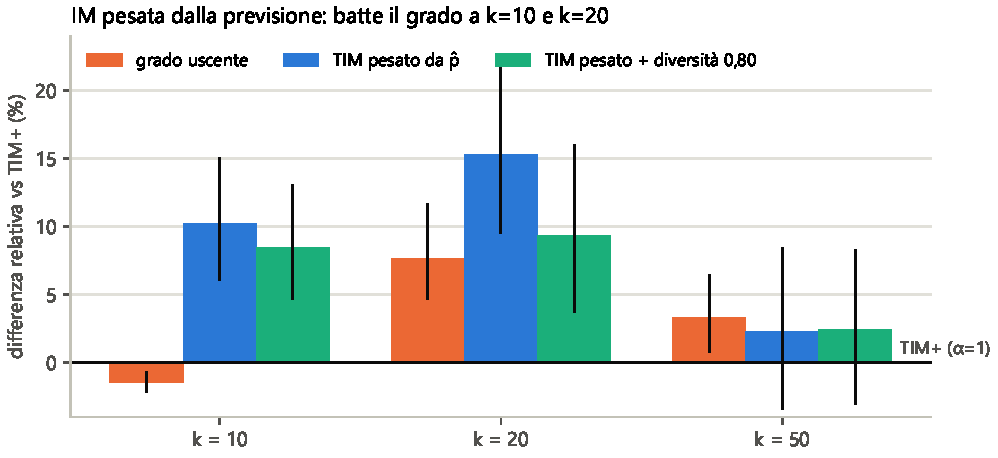
\includegraphics[width=\textwidth]{fig_im_pesata}
    \end{column}
    \begin{column}{0.43\textwidth}
      \small
      Contro il grado, direttamente:\\[0.3em]
      \begin{tabular}{@{}lrr@{}}
        \toprule
        $k$ & TIM pesato & $p$ \\
        \midrule
        10 & \pos{$\mathbf{+11{,}85\%}$} & $<0{,}001$ \\
        20 & \pos{$\mathbf{+7{,}06\%}$} & $<0{,}001$ \\
        50 & $-1{,}01\%$ & 0,73 \\
        \bottomrule
      \end{tabular}\\[0.6em]
      Sceglie \textbf{pochi seed gi\`a attivi}: 7 su 20, contro 20 su 20 di TIM+. Trova chi non parla ancora dell'evento ma raggiunge chi adotter\`a.\\[0.6em]
      Un'AUC di 0,68 basta: il peso non deve essere buono, deve essere \emph{meglio dell'uniforme}.
    \end{column}
  \end{columns}
\end{frame}

% =====================================================================
\begin{frame}{Che cosa non ha funzionato}
  \centering
  \setlength{\tabcolsep}{8pt}
  \renewcommand{\arraystretch}{1.7}
  \begin{tabular}{|>{\raggedright\arraybackslash}m{0.31\textwidth}|>{\raggedright\arraybackslash}m{0.60\textwidth}|}
    \hline
    \rowcolor{tenue}\textbf{componente} & \textbf{esito, e come \`e stato verificato} \\
    \hline
    TIM+ non pesato & \textcolor{bordeaux}{perde col grado} da $k=20$ in su, $p \le 0{,}001$ \\
    \hline
    GNN sugli archi, per i seed & stima $p$ l'86\% meglio, ma nessun vantaggio coerente sui seed: tre budget, tre risposte \\
    \hline
    loss pesata sugli hub & respinta su \textbf{entrambi} i substrati, $-2{,}1\%$ e $-2{,}0\%$ \\
    \hline
    R-SIGN & la struttura relazionale informa gli alberi ($p=0{,}006$), non la GNN ($p=0{,}22$) \\
    \hline
    fusione convenzionale & $-0{,}15$ di $\Qtras$, $p<0{,}001$: il multistrato paga solo tarato \\
    \hline
    escludere i gi\`a attivi & da $-59\%$ a $-81\%$: toglie esattamente chi conta \\
    \hline
    potere esplicativo assoluto & \textcolor{bordeaux}{678 adozioni su 269.081}, lo 0,3\%: lo shock \`e esogeno, il modello lo misura ($\times 4{,}55$) ma non lo contiene \\
    \hline
  \end{tabular}
\end{frame}

% =====================================================================
\begin{frame}{Le due tesi}
  \begin{columns}[T]
    \begin{column}{0.48\textwidth}
      \begin{block}{Il substrato decide, e si pu\`o sapere prima}
        \small Prima di costruire qualunque cosa basta una misura semplice --- i vicini contano davvero, o \`e solo il grado? --- e la risposta dice gi\`a se il resto del lavoro trover\`a qualcosa.\\[0.4em]
        StackExchange: \male{$-0\%$}, ogni componente nulla.\\
        Higgs: \pos{$+73\%$}, le stesse componenti danno segnale.\\[0.4em]
        Una pipeline con risultati positivi su entrambi sarebbe \emph{meno} credibile.
      \end{block}
    \end{column}
    \begin{column}{0.48\textwidth}
      \begin{block}{Prevedere prima di ottimizzare}
        \small Chi massimizza \emph{quanti} nodi perde contro il grado. Chi sa \emph{chi} adotter\`a --- anche solo un po', AUC 0,68 --- lo batte.\\[0.4em]
        Sapere \emph{come} si trasmette ($p$ sugli archi) non ha pagato sui seed; sapere \emph{a chi} ($\phat$ sui nodi) s\`i.\\[0.4em]
        Le comunit\`a sono il pezzo di conoscenza che pesa di pi\`u.
      \end{block}
    \end{column}
  \end{columns}
  \vspace{0.8em}
  \centering\small\color{grigio}
  Quello che ci portiamo via \`e soprattutto un modo di lavorare: decidere il criterio prima di vedere i dati, giudicare sulle adozioni vere e non sulle simulazioni, mettere accanto a ogni numero quanto rumore c'\`e, e raccontare anche ci\`o che non ha funzionato.
\end{frame}

% =====================================================================
\begin{frame}[plain]
  \centering
  \vfill
  {\fontsize{30}{36}\selectfont\bfseries\color{petrolioscuro}Grazie per l'attenzione}\\[1.2em]
  {\color{grigio}Davide Cinelli \textperiodcentered{} Giuseppe Cuiuri}
  \vfill
\end{frame}

\end{document}
